\documentclass[runningheads]{llncs}

\usepackage[T1]{fontenc}
\usepackage{graphicx}
\usepackage{xparse} % interval

% to display URLs in blue roman font according to Springer's eBook style:
%\usepackage{color}
%\renewcommand\UrlFont{\color{blue}\rmfamily}
%\urlstyle{rm}

\begin{document}
\title{Computer Networks Project: \\ Romanian Railways}

\author{P. Braha\inst{1}\orcidID{0009-0001-3636-2455}}
\authorrunning{P. Braha}
\institute{Alexandru Ioan Cuza University, Iasi IS 700221, Romania
\email{petrubraha@gmail.com}\\
\url{https://github.com/petru-braha}}

\maketitle

\begin{abstract} This work contains an overview of the client-server paradigm offering, to the public transport companies, a concrete (and open source) informational system connected with potential clients. This system provides a service that notifies the consumers about the traveling schedule, the available means of transport (e.g. trains) associated with their time and location, and other related knowledge such as status of departure/arrival and vehicle identification. Any user can report late arrivals, but in a controlled manner such that the misleading records are checked and ignored, if necessary. The application runs concurrently and achieves great communication speed with the customers and good quality of the responses delegated. The security of the system is accomplished by having two different running servers at different locations. If one of them fails, there exists a guaranteed backup. Their communication is not omitted. This paper represents an implementation reference for the field of network programming and management.

\keywords{Server \and Client \and Concurrency \and Transport level \and I/O multiplexing \and Commands \and Threads \and Sockets }
\end{abstract}

%%------------------------------------------------
%%------------------------------------------------

\section{Introduction}

"Romanian Railways" is a project which involves compilation of two programs: one for the server and the other for client(s). It is in a professionally working state when two "server.c" instances are concurrently running indefinitely. One of such instance could manage x number of clients, where $x \in \left[0, 1024\right]$ (this limitation is later disclosed in the chapter 4). 

The current document continues to explain the requirements of such a system, the logic behind it, and the real use cases. Within the next section, a short list of the adopted technologies can be explored. Choosing the right tools will determine the overall quality of the apps. In the third chapter, you may find the structure of the server application, and some illustrations of the routines executed. Following this, additional details, experiments, and observations are analyzed. The advantages and roles of the decisions took regarding the implementation are discussed too. This part creates an opening of the API definitions at application level. The conclusions will summarize my project and propose some scenarios where the "RR application" could be useful.

\subsection{Motivation}

The entire repository is a matter of personal interest for the "Computer Networks" course. Officially, it is known as a laboratory homework, but the main goal is far higher: to be a contribution in practical life. Being encouraged to provide a creative solution, this project was designed.

%%------------------------------------------------
%%------------------------------------------------

\section{Applied Technologies}

Three main core objectives were followed in the development: speed, correctness and security. Therefore C programming language was elected because:
\begin{itemize}
    \item it is one of the fastest compiled language 
    \item it supplies network management resources, such as threads and sockets
    \item it delivers simple syntax, yet highly customizable flags and options (very important in the current implementation - see non-blocking calls)
    \item it has all the necessary tools to assure the objectives previously considered; a more advanced language like C++ would add an layer of unnecessary complexity
\end{itemize}

The server has to be concurrent for reasons later argued. To attain this, threads were selected to handle this requirement; they are a multiple-purpose mechanism, as we'll observe in the final composition of the program. Last but not least, the exchange of messages between the customers and the server are realized with sockets.

%%------------------------------------------------
%%------------------------------------------------

\section{Application Structure}

Expose the concepts used in modeling and present a detailed diagram of the application.

zic doar ce am folosit iar in urmatorul zic  de ce am folosit
    
\begin{figure}[!h]
    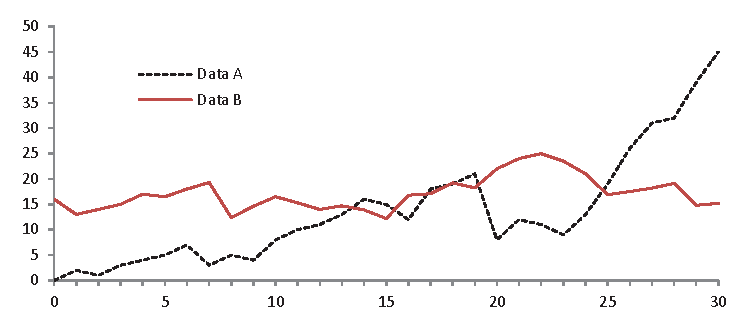
\includegraphics[width=\textwidth]{fig1.eps}
    \caption{Execution diagram} \label{fig1}
\end{figure}

%%------------------------------------------------
%%------------------------------------------------

\section{Implementation Aspects}

The base of the current code follows the TCP stack model, but with a refined blueprint, outlined in the following subsections. 

\subsection{Concurrency schema}

The server application must be concurrent, otherwise a queue of clients would be formed and their requests will be delivered slowly. The following list of strategies were evaluated in our build:
\begin{itemize}
    \item pre-forked execution 
    \item pre-threaded execution 
    \item child process per client
    \item thread per client
\end{itemize}

Using threads over child processes is due to their "shared memory" character (please also note: \cite{fork-vs-thread}). Even if a child process is "copy on write" optimized, it is not the best choice for a long-term running server which frequently updates all of the data. 
The final configuration is a combination of the second and forth approaches. In the server starts prethreaded execution responsable of efficient operations, and adds threads for each new connected client. More about the benefits of this technique are presented in the aspects of the implementation (forth section).

\subsection{Transport protocol}

The transport layer uses a combination of TCP and UDP, where their advantages were exploited for the appropriate situations in the code.
The TCP protocol is used for the commands that influence the server's data. Being a secure protocol, TCP provides acknowledgments for all the transmitted messages. However, it implies an increased amount of time, which proposes the usage of the UDP protocol. TCP is a robust mechanism which assures correctness of transmissions, which is mandatory for clients' reports. But, in cases of simpler queries, it is preferred a faster communication. If the communication fails, it can be simply readdressed by the consumer (see the forth chapter regarding how wrong outputs were avoided).
Briefly, the clients use TCP when sending requests to change the trains' schedule, and UDP for information retrieval.

\subsection{I/O Multiplexing}

This is a new topic, which further improves the speed of the client-server correspondence. The select() primitive with unblocking I/O operations is considered the fastest strategy, (accordingly to \cite{non-block-select} and \cite{course}. What is better than an iterative server with I/O multiplexing? A concurrent one, which uses the same principle.



What about "prethreaded" approach? It could In the future I want to keep up multiple server instances, not just two. Pre-threaded approach could work if all the machines have a not mimum number of cores/threads. Since I can not gurantee on which type of machine.Complicated code. If more clients are connecting.

explain prethreaded threads
explain 

Acceptance of clients is concurrent. Serving them iteratively VS concurently test.

extra server for security
administrator login

innovative sections of the project code 
describe the api - describe real usage scenarios.

\subsection{Experiment}

High cost operation times (both TCP and UDP commands) for:
\begin{itemize}
    \item sequentially serving
    \item concurrently serving
\end{itemize}

\begin{table}
    \caption{Results: of costly operations on local clients.}\label{tab1}
    \begin{tabular}{|l|l|l|}
    \hline
    Heading level &  Example & Font size and style\\
    \hline
    Title (centered) &  {\Large\bfseries Lecture Notes} & 14 point, bold\\
    1st-level heading &  {\large\bfseries 1 Introduction} & 12 point, bold\\
    2nd-level heading & {\bfseries 2.1 Printing Area} & 10 point, bold\\
    3rd-level heading & {\bfseries Run-in Heading in Bold.} Text follows & 10 point, bold\\
    4th-level heading & {\itshape Lowest Level Heading.} Text follows & 10 point, italic\\
    \hline
    \end{tabular}
    \end{table}
    

\subsection{Definitions and Decisions}



- estimated times = initial times defined by the generated schedule
- confirmed times = estimated times +/- delays (depends if the train arrives earlier or later)
- status has two fields - each indicates whether it has left or arrived
- a clear distinction is made between the word estimated and confirmed. The former has an information initializing character, and while the server is running for that day estimated emphasizes that the information

The time of the application is the current Romania time.
- an itinerary is from point A to point B and no other points exists between these two. If that would be the case then extra complexity would be added to the logic of the application.

- locations types
    - departures
    - arrivals

- times types
    - confirmed departure time
    - estimated departure time
    - confirmed arrival time
    - estimated arrival time


\subsection{Application protocol}

The data is composed of:
\begin{itemize}
    \item routes
    \item departure/arrival status
    \item delays
    \item arrival estimation
\end{itemize}

The server is responsable for:
\begin{itemize}
    \item sends data to clients
    \item receives data from xml files
    \item receives delays from clients
    \item updates dalays, arrival estimation

\end{itemize}
    
The client application contains 5 commands presented below. The function model is return\_type name\_function parameter(s).

\begin{itemize}
    \item $[id\_train, time\_departure\_estimated, time\_arrival\_estimated, status]$ routes(location\_departure, location\_arrival);
    \item [id\_train, time\_departure\_confirmed, location\_arrival] departures(location\_departure);
    \item [id\_train, time\_arrival\_confirmed, location\_departure] arrivals(location\_arrival);
    \item void report(id\_train);
    \item void quit();
\end{itemize}

%%------------------------------------------------
%%------------------------------------------------

\section{Conclusions}

speed:
concurrency
tcp/udp - transport level
i/o multiplexing with non-blocking calls

corectness:
tcp protocol

durability:
extra server

\begin{credits}
    \subsubsection{\ackname} A bold run-in heading in small font size at the end of the paper is
    used for general acknowledgments, for example: This study was funded
    by X (grant number Y).
    e
    \subsubsection{\discintname}
    It is now necessary to declare any competing interests or to specifically
    state that the authors have no competing interests. Please place the
    statement with a bold run-in heading in small font size beneath the
    (optional) acknowledgments\footnote{If EquinOCS, our proceedings submission
    system, is used, then the disclaimer can be provided directly in the system.},
    for example: The authors have no competing interests to declare that are
    relevant to the content of this article. Or: Author A has received research
    grants from Company W. Author B has received a speaker honorarium from
    Company X and owns stock in Company Y. Author C is a member of committee Z.
    \end{credits}
    

%%------------------------------------------------
%%------------------------------------------------
%citations: square brackets and consecutive numbers. Citations using labels or the author/year
%convention are also acceptable. The following bibliography provides
%a sample reference list with entries for journal
%aarticles~\cite{ref_article1}, an LNCS chapter~\cite{ref_lncs1}, a
%abook~\cite{ref_book1}, proceedings without editors~\cite{ref_proc1},
%aand a homepage~\cite{ref_url1}. \cite{ref_article1,ref_book1,ref_proc1,ref_url1}.

% \bibliographystyle{splncs04}
% \bibliography{mybibliography}

\begin{thebibliography}{8}
\bibitem{fork-vs-thread}Sysel, Martin. "A comparison of processes and threads creation." Software Engineering Perspectives in Intelligent Systems: Proceedings of 4th Computational Methods in Systems and Software 2020, Vol. 1 4. Springer International Publishing, 2020. 
%\url{https://doi.org/10.1007/978-3-030-63322-6_85}

\bibitem{non-block-select} Stevens, W. Richard, Andrew M. Rudoff, and Bill Fenner. Unix network programming volume 1: the sockets networking API. Vol. 3. Boston: Addison-Wesley Professional, 2003.

\bibitem{course}
  Croitoru Eugen. "Computer Networks" course page. Alexandru Ioan Cuza University, 2024. \\
  \url{https://profs.info.uaic.ro/eugen.croitoru/teaching/ga/}

\bibitem{udp-connect}
\url{https://stackoverflow.com/questions/9741392/can-you-bind-and-connect-both-ends-of-a-udp-connection}

\bibitem{ref_article1}
Author, F.: Article title. Journal \textbf{2}(5), 99--110 (2016)

\bibitem{ref_lncs1}
Author, F., Author, S.: Title of a proceedings paper. In: Editor,
F., Editor, S. (eds.) CONFERENCE 2016, LNCS, vol. 9999, pp. 1--13.
Springer, Heidelberg (2016). \doi{10.10007/1234567890}

\bibitem{ref_book1}
Author, F., Author, S., Author, T.: Book title. 2nd edn. Publisher,
Location (1999)

\bibitem{diagram-site} ccaaca \url{https://sequencediagram.org/}

\bibitem{ref_proc1}
Author, A.-B.: Contribution title. In: 9th International Proceedings
on Proceedings, pp. 1--2. Publisher, Location (2010)

\bibitem{ref_url1}
LNCS Homepage, \url{http://www.springer.com/lncs}, last accessed 2023/10/25
\end{thebibliography}
\end{document}